\documentclass[UTF8,a4paper,12pt]{ctexart}
\usepackage[margin=23mm]{geometry}
\usepackage{graphicx,longtable,booktabs,array,xcolor,colortbl,float,xurl,needspace}
\usepackage[unicode,colorlinks=true,linkcolor=black,urlcolor=blue]{hyperref}
\setmainfont{Times New Roman}
\definecolor{reportblue}{HTML}{18344D}
\definecolor{reportpale}{HTML}{EDF4F7}
\ctexset{section={format=\Large\bfseries\raggedright}}
\setlength{\parskip}{0.35em}
\setlength{\parindent}{2em}
\linespread{1.18}
\pagestyle{plain}
\emergencystretch=2em
\hypersetup{pdftitle={自研RISC-V二维图形SoC},pdfauthor={}}
\begin{document}
\begin{center}
{\LARGE\bfseries 自研RISC-V二维图形SoC}\par
\vspace{0.7em}
{\large AMD自主选题专项设计报告}\par
2026年11月3日
\end{center}


\Needspace{12\baselineskip}\section{选题背景与创新点}

\Needspace{8\baselineskip}\subsection{应用背景与设计目标}

本作品面向 FPGA 软硬件协同教学与二维交互应用，在 ALINX AX7020 的 Zynq XC7Z020CLG400-2 上构建可加载 C 程序的图形系统。系统将处理器计算、批量像素绘制、显示扫描、输入和音频整合，通过 CPU 基准、固定图形负载及两款交互应用验证设计效果。\par

小型软核逐像素绘制会占用较多指令和总线周期，而完整 800×600 RGB332 画面需要 480000 字节，超过单个片上暂存区容量。本设计分别从处理器执行效率和图形存储组织入手，将控制判断交给软核，将重复像素操作交给专用硬件，并通过两带复用在有限 BRAM 中生成完整画面。\par

\Needspace{8\baselineskip}\subsection{已有工作与自主贡献}

本作品以开放指令集和 FPGA 图形技术为基础，参考 PicoRV32、Project F 等公开项目的设计思路，自主实现流水处理器微架构、图形命令与分带提交通路，以及可加载应用、外设和资源管理系统，形成计算、绘制、显示与交互协同运行的完整作品。\par

核心创新集中于三方面：预测、旁路及条件双指令路径协同提升软核执行效率；以 256 KiB 暂存区复用实现原生 800×600 图形生成；通过整帧提交、独立像素参考和逐扫描计数将图形正确性与持续性能统一验证。这些设计共同体现资源受限 FPGA 上的系统级协同优化。\par

作品明确区分自主系统设计与第三方应用资源：处理器、图形与运行管理为技术主体，标准基准与交互场景用于形成可复现的综合负载；字体、音乐和美术保留来源清单，便于复现和后续扩展。\par

\Needspace{12\baselineskip}\section{设计原理与功能框图}

\Needspace{8\baselineskip}\subsection{系统总体结构}

PS ARM 运行 Linux/PYNQ，承担程序加载、USB 事件采集、PCM 数据补给和物理内存管理；PL 自研 RISC-V 执行裸机 C 应用，图形模块完成批量像素处理。DDR 保存程序、素材和显示双帧缓冲，HDMI 从已提交的前台帧读取数据。\par

\begin{figure}[H]
\centering
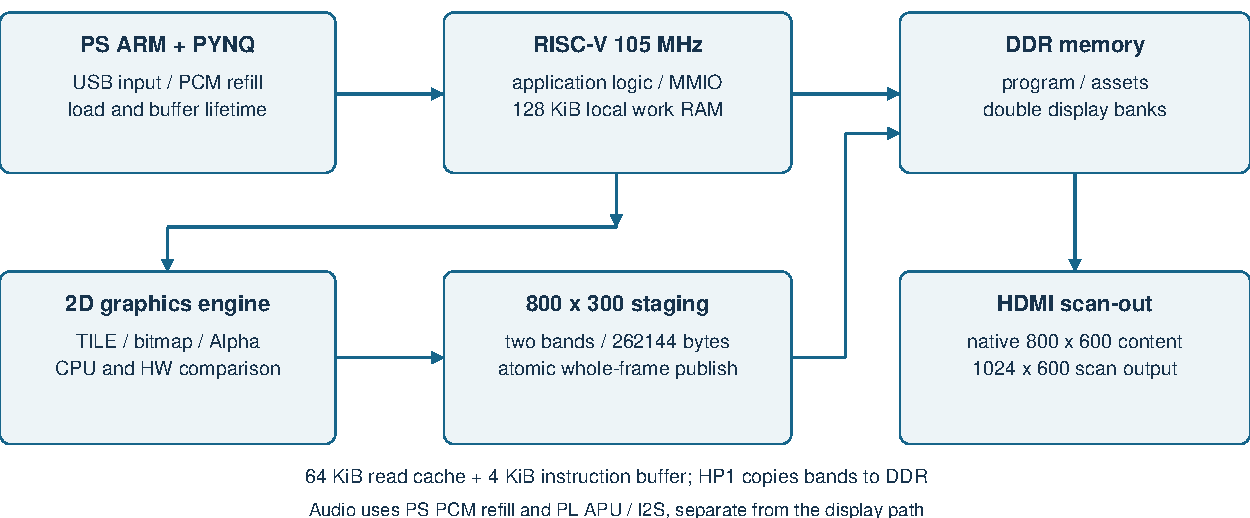
\includegraphics[width=\linewidth]{figures/architecture.pdf}
\caption{系统总体结构与主要数据流}
\end{figure}

实际应用画布为 800×600 RGB332，居中于 1024×600 HDMI 扫描区域，左右各留 112 像素。CPU 与图形工作频率为 105 MHz，视频串行时钟为 525 MHz。两者承担不同任务，性能统计使用 CPU 实际时钟。\par

\Needspace{8\baselineskip}\subsection{处理器与存储结构}

处理器采用注册取指、译码队列、执行、访存和写回五个主流水级，结合动态分支预测、间接目标缓存、预译码与结果旁路，减少控制转移和数据相关带来的等待。共享取指与数据通路采用明确仲裁，被重定向的旧取指响应先排空，再复用请求状态。\par

\begin{figure}[H]
\centering
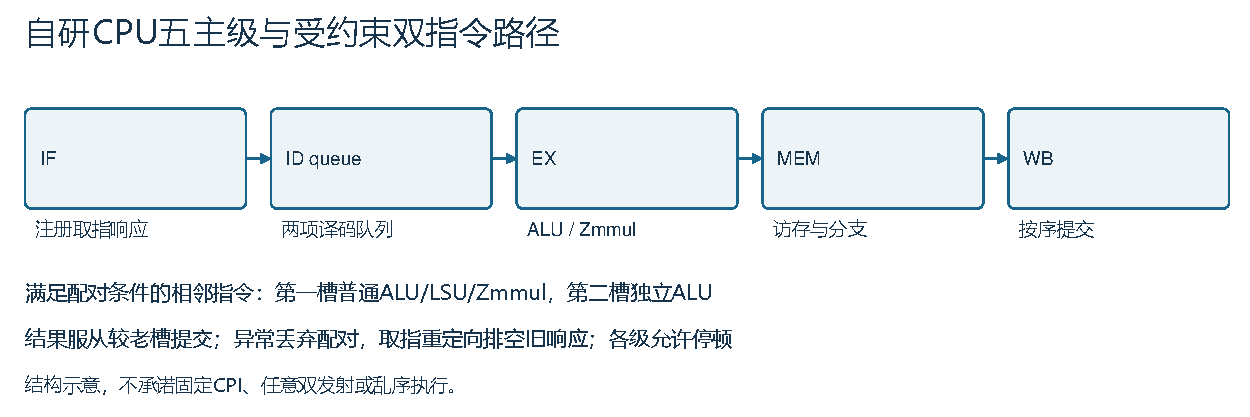
\includegraphics[width=\linewidth]{figures/cpu_pipeline.pdf}
\caption{五主级流水与受约束双指令路径}
\end{figure}

处理器对满足对齐、数据独立性和操作类型条件的相邻指令启用第二 ALU 槽，两项结果依照程序顺序提交并处理异常。条件双指令执行与预测、旁路共同减少指令等待，指令集采用 RV32I 与 Zmmul 乘法扩展。\par

DDR 程序和只读素材通过 64 KiB 四路缓存访问，缓存行大小为 64 字节；4 KiB 指令缓冲改善取指局部性，128 KiB BRAM 保存工作数据与栈。只有 AXI 传输成功结束后，缓存行才被发布为有效；错误、刷新和暂停状态下阻止不完整行进入执行路径。工作数据与栈使用独立片上 RAM 路径。\par

\Needspace{8\baselineskip}\subsection{图形加速与完整帧提交}

CPU 通过内存映射寄存器提交矩形填充、TILE、DDR 位图、裁剪、翻转、透明色和 Alpha 命令。Alpha 支持 0\%、25\%、50\%、75\%、100\% 五档。软件比较模式由 CPU 执行像素运算，其接口要求的暂存区初始化成本同样计入测试。\par

\begin{figure}[H]
\centering
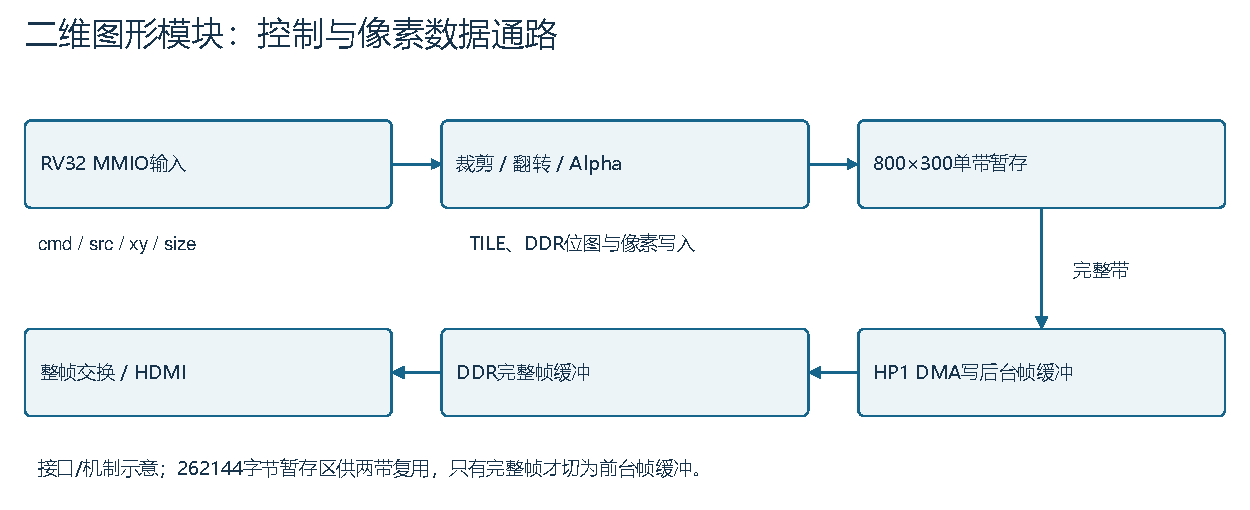
\includegraphics[width=\linewidth]{figures/gpu_datapath.pdf}
\caption{图形控制 暂存 搬运与显示数据通路}
\end{figure}

单带为 800×300、240000 字节，可放入 262144 字节暂存区。系统先绘制上带并搬入 DDR 后台帧，再复用同一暂存区绘制和搬运下带。控制模块仅在两带全部完成且到达显示帧边界时交换前后台，避免扫描到尚未完成的半帧；双行缓存用于缓冲显示侧短时总线波动。\par

\begin{figure}[H]
\centering
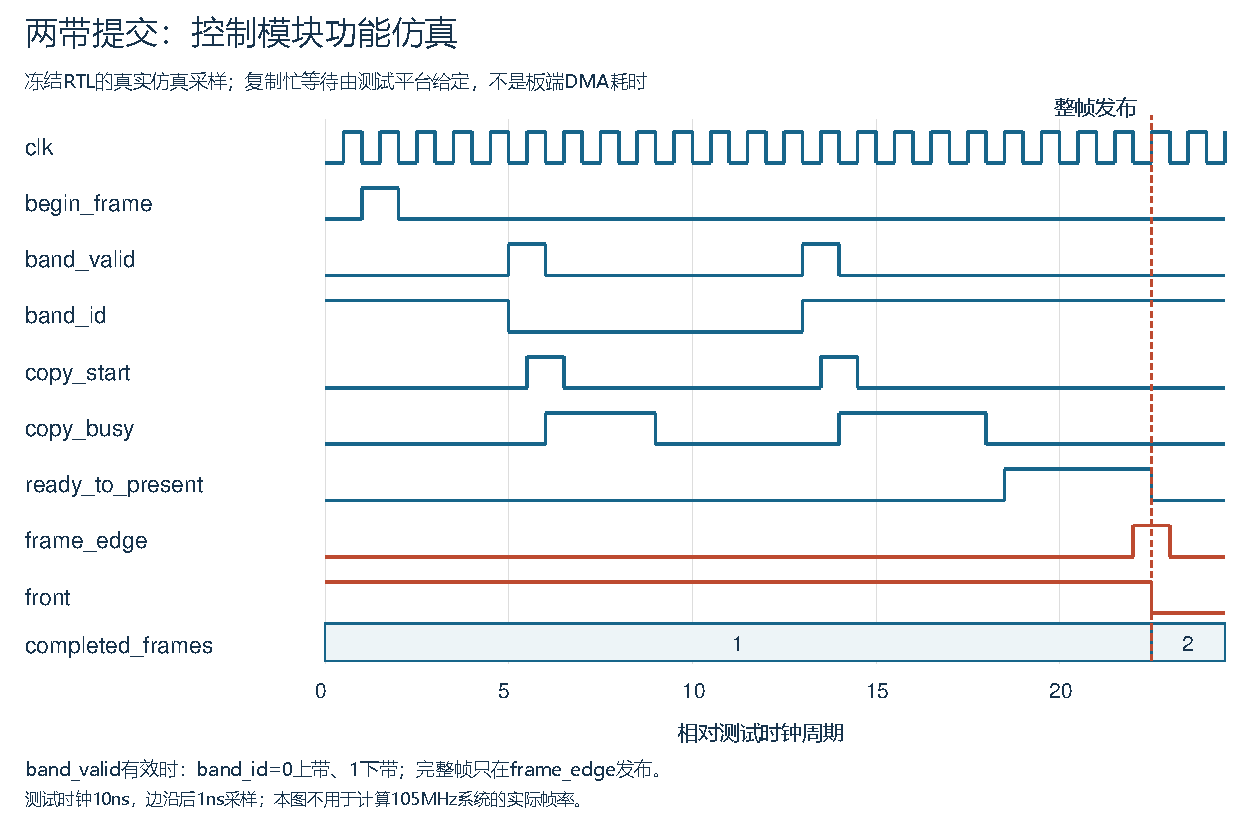
\includegraphics[width=\linewidth]{figures/two_band_sequence.pdf}
\caption{两带提交控制模块功能仿真时序}
\end{figure}

功能仿真验证了上带搬运、下带搬运和显示帧边界切换之间的完整时序，整帧提交将绘制进度与前台扫描明确衔接。双行缓存进一步缓冲 DDR 访问波动，支持连续显示。\par

\Needspace{12\baselineskip}\section{软硬件划分依据与接口设计}

\Needspace{8\baselineskip}\subsection{分工依据}

应用状态更新、菜单判断与负载选择包含较多条件分支，适合使用 C 程序由软核执行；填充、位图读取和透明混合具有重复像素运算特征，使用专用硬件降低指令开销。PS 利用现有 Linux USB 与文件系统支持管理外设和素材，应用逻辑及图形生成保持在 PL 侧。\par

{\small\setlength{\tabcolsep}{4pt}\renewcommand{\arraystretch}{1.3}

\begin{longtable}{>{\raggedright\arraybackslash}p{0.2\linewidth}>{\raggedright\arraybackslash}p{0.38\linewidth}>{\raggedright\arraybackslash}p{0.34\linewidth}}

\toprule

\textbf{功能} & \textbf{实现位置} & \textbf{主要输入与输出} \\ \midrule

\endfirsthead

\toprule

\textbf{功能} & \textbf{实现位置} & \textbf{主要输入与输出} \\ \midrule

\endhead

应用逻辑 & PL RISC-V & 统一输入状态 → 绘图及音频控制命令 \\

像素运算 & PL 图形模块 & 参数与素材 → 暂存带像素 \\

显示提交 & PL 搬运与扫描模块 & 完整两带 → DDR 前台帧与 HDMI \\

外设与加载 & PS ARM & USB、文件 → 输入寄存器与程序内存 \\

音频播放 & PS 补给、PL I²S & PCM 数据 → 数字音频串行输出 \\

\bottomrule

\end{longtable}

}

\Needspace{8\baselineskip}\subsection{存储与控制接口}

{\small\setlength{\tabcolsep}{4pt}\renewcommand{\arraystretch}{1.3}

\begin{longtable}{>{\raggedright\arraybackslash}p{0.45\linewidth}>{\raggedright\arraybackslash}p{0.45\linewidth}}

\toprule

\textbf{地址区域} & \textbf{功能} \\ \midrule

\endfirsthead

\toprule

\textbf{地址区域} & \textbf{功能} \\ \midrule

\endhead

0x80000000，16 MiB 窗口 & 程序与只读素材 \\

0x20000000，128 KiB & 工作 RAM 与栈 \\

0x10000100 & 应用状态与控制 \\

0x10000200 & 图形命令与状态 \\

0x10000300 & 音频控制 \\

0x43c00000 & PS 控制窗口 \\

\bottomrule

\end{longtable}

}

软件分别组织菜单、两个 CPU 配置、三类图形基准和两款交互应用。每个程序保留独立构建配方，防止公共代码调整后无法重现对应测试程序。\par

\Needspace{8\baselineskip}\subsection{输入 音频与资源生命周期}

手柄、触屏和鼠标事件由 PS 统一采集。触屏双击结合时间、位置和当前页面判定，鼠标采用按键边沿触发；应用切换时清理未完成手势。主菜单为六入口单排布局，手柄、触屏与鼠标均可完成进入和返回。\par

\begin{figure}[H]
\centering
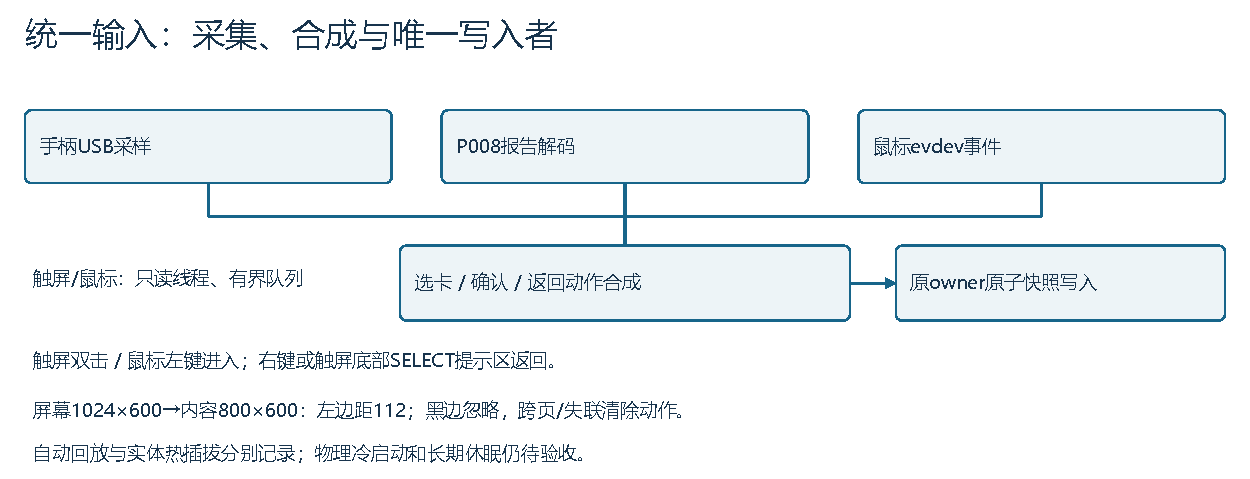
\includegraphics[width=\linewidth]{figures/input_flow.pdf}
\caption{统一输入采集与事件处理}
\end{figure}

\begin{figure}[H]
\centering
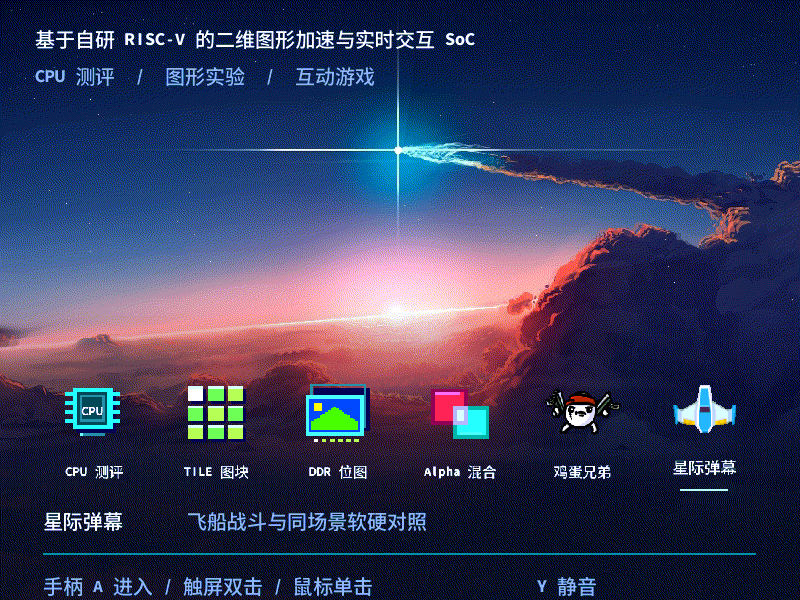
\includegraphics[width=\linewidth]{screenshots/12_main_menu_cloud_dock.png}
\caption{主菜单板端运行画面}
\end{figure}

多外设管理结合设备识别、输入优先级和重连调度，协调手柄、触屏与鼠标接入统一控制接口。实物操作覆盖三种输入的应用进入、返回及手柄启动后的输入接续，体现完整的人机交互能力。\par

音频采用 32 kHz、单声道、有符号 16 位 PCM。PS 补给 FIFO，PL 完成播放与 I²S 输出，经 MAX98357A 音频放大器驱动扬声器。自制洞洞板使用双排母连接开发板接口与商购音频模块；配套扬声器标称规格为 3 W、8 Ω。\par

\begin{figure}[H]
\centering
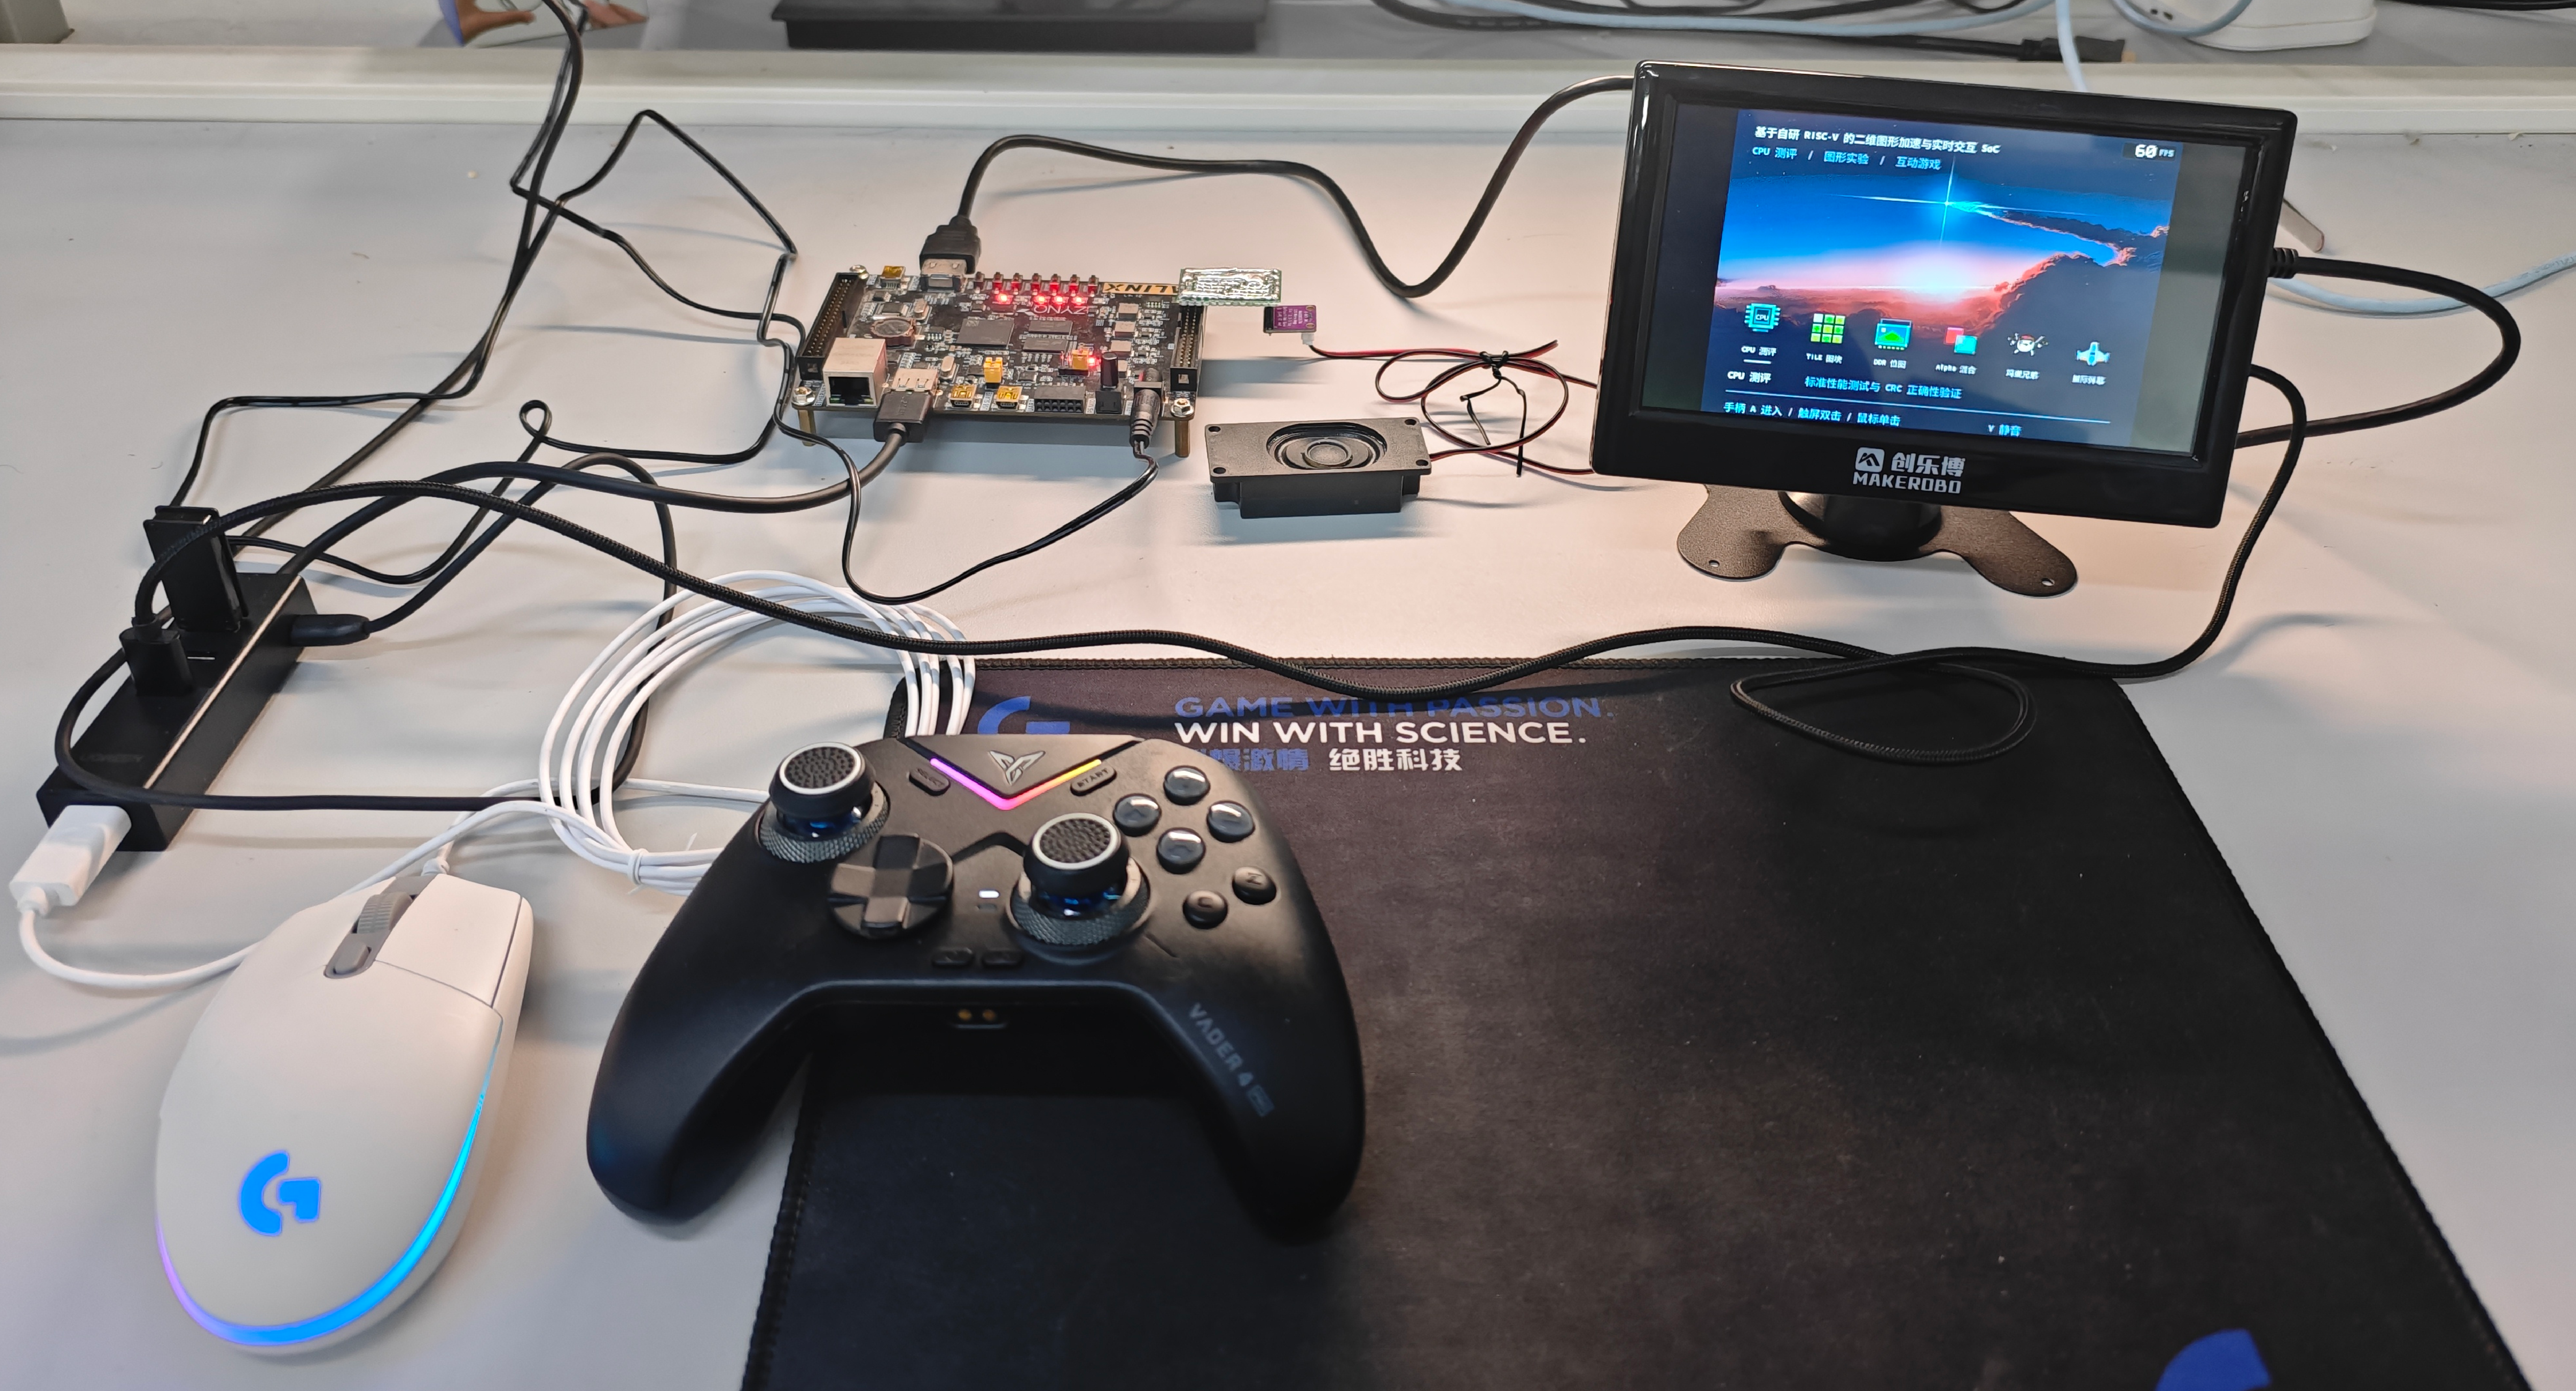
\includegraphics[width=\linewidth]{photos/01_system_overview.pdf}
\caption{整机与外设连接实物}
\end{figure}

\begin{figure}[H]
\centering
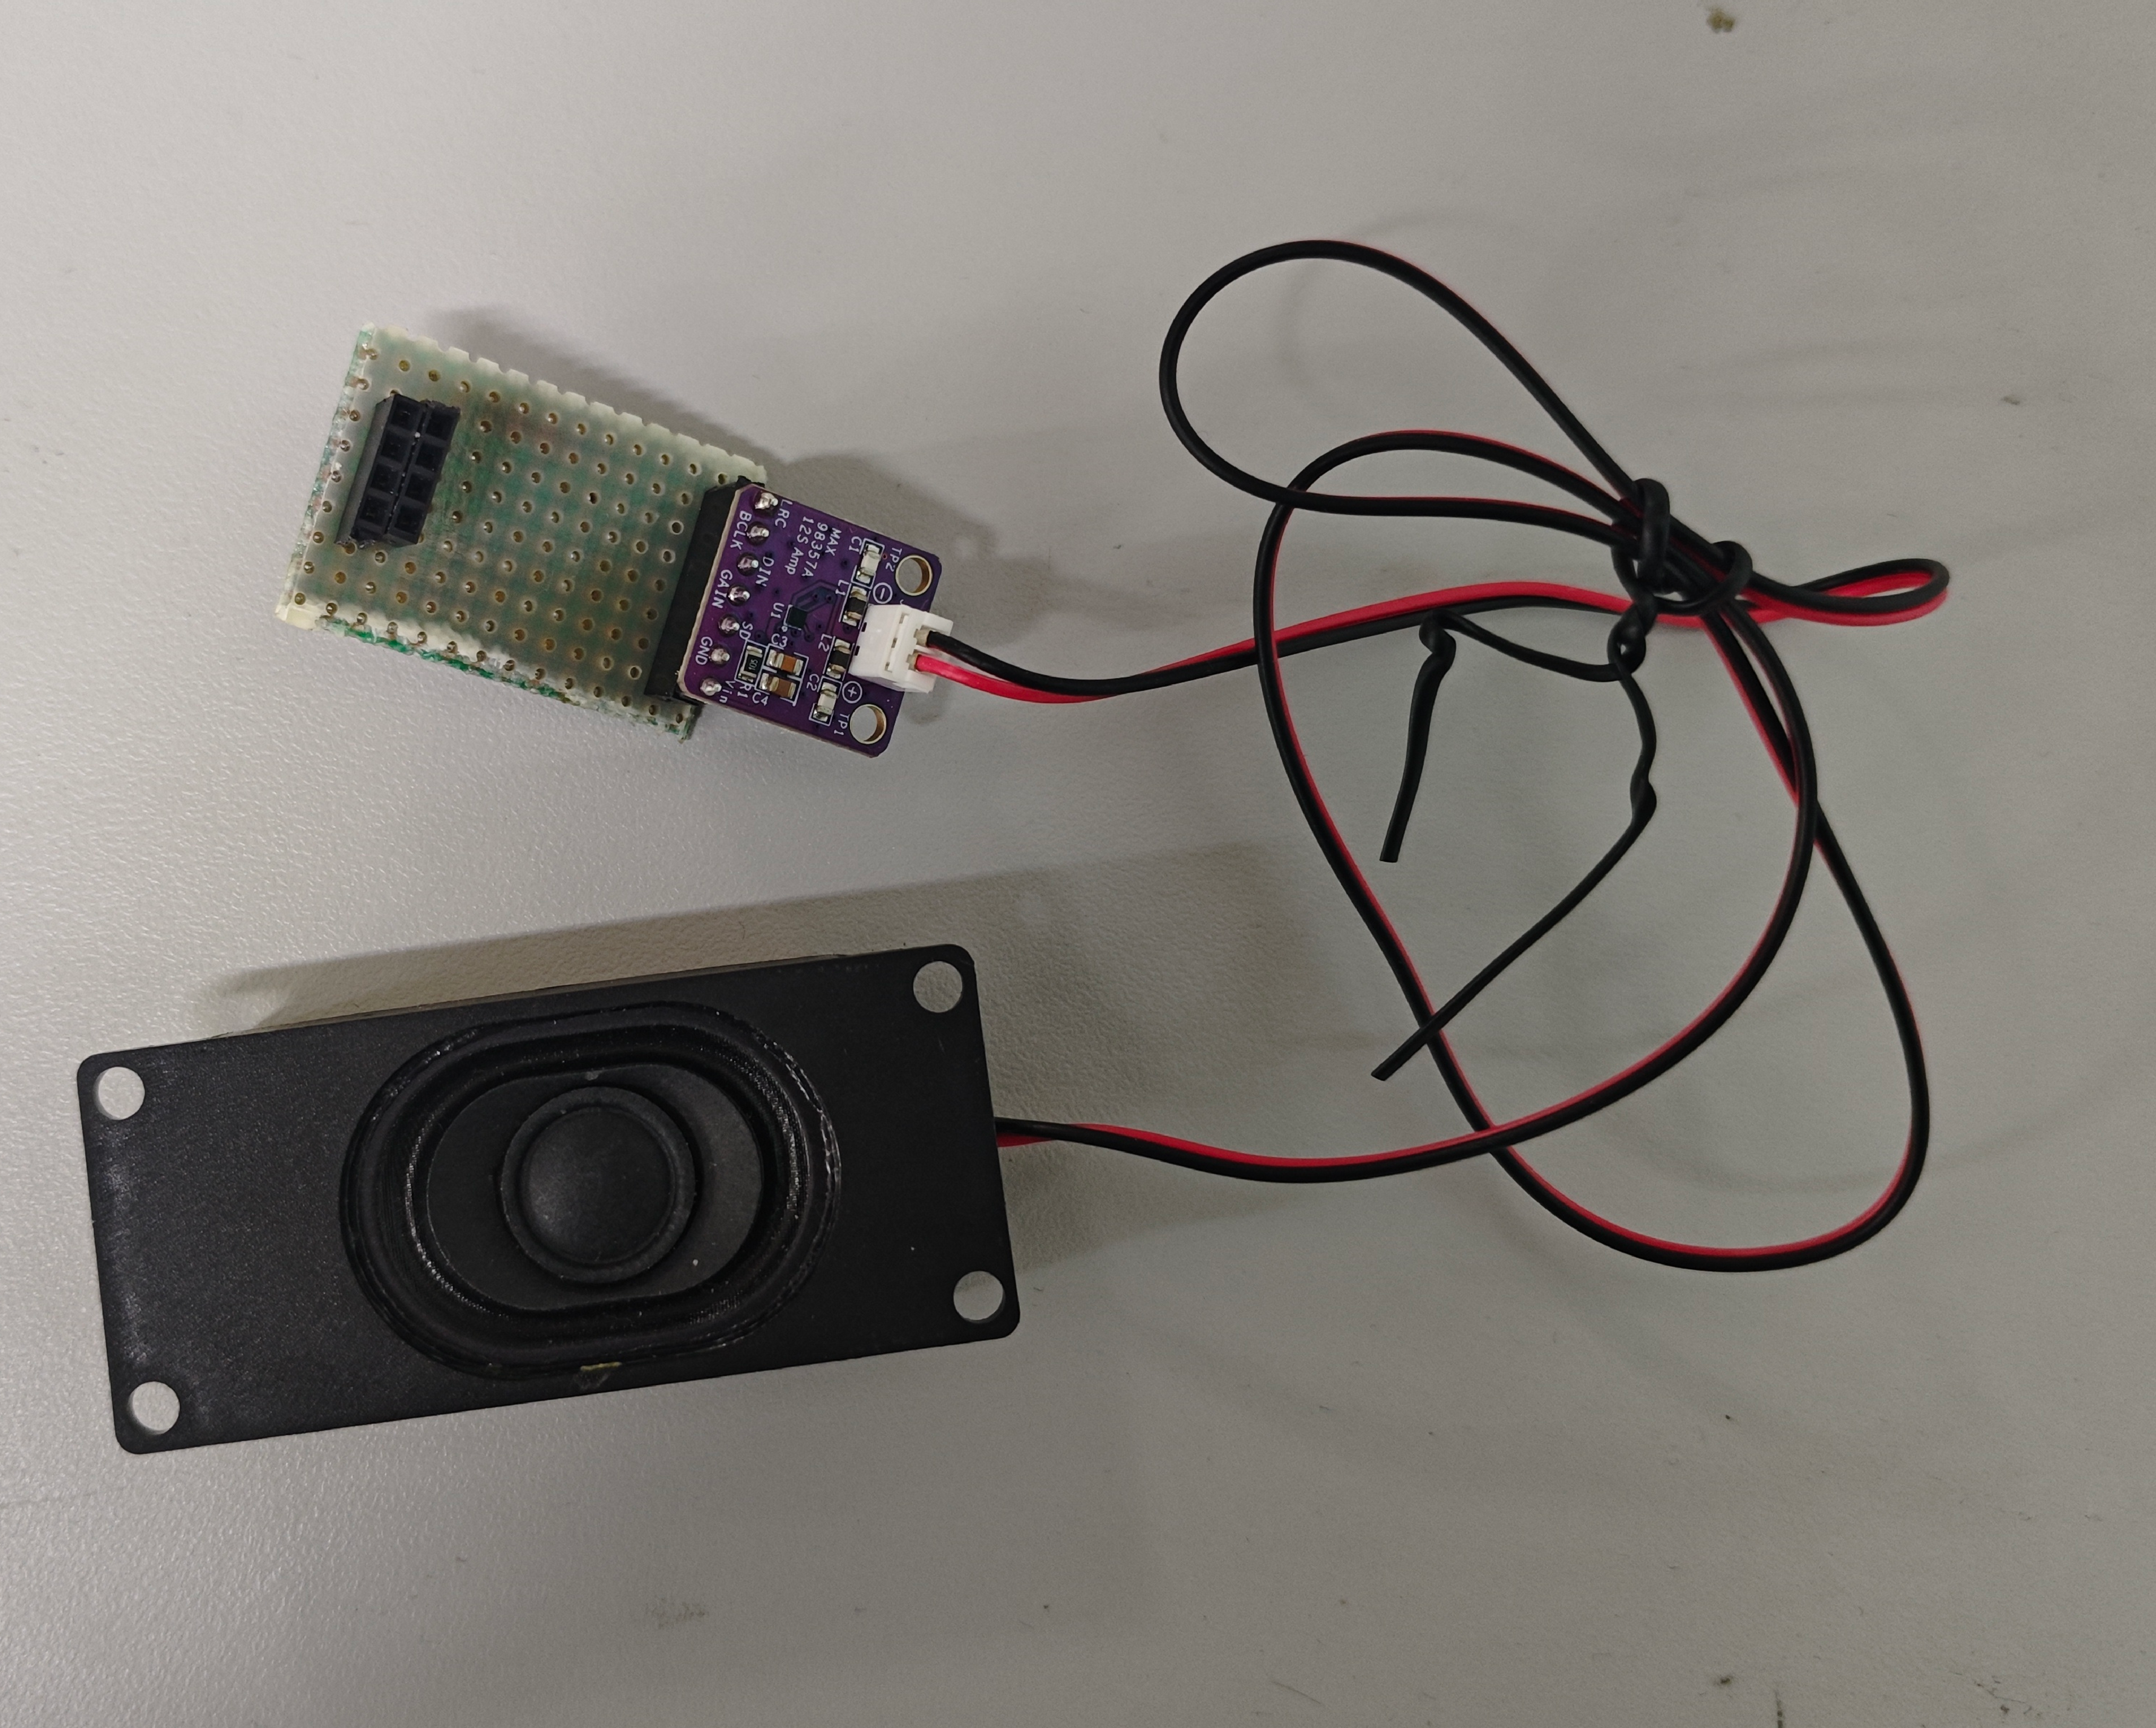
\includegraphics[width=\linewidth]{photos/05_adapter_top.pdf}
\caption{自制I²S转接板与MAX98357A模块}
\end{figure}

应用切换采用完整的退出握手：请求当前应用完成帧提交与退出确认，协调音频暂停及搬运排空，再暂停软核并释放内存。按生产者与消费者依赖组织交接，使程序、图像和音频资源具有一致的生命周期。\par

\begin{figure}[H]
\centering
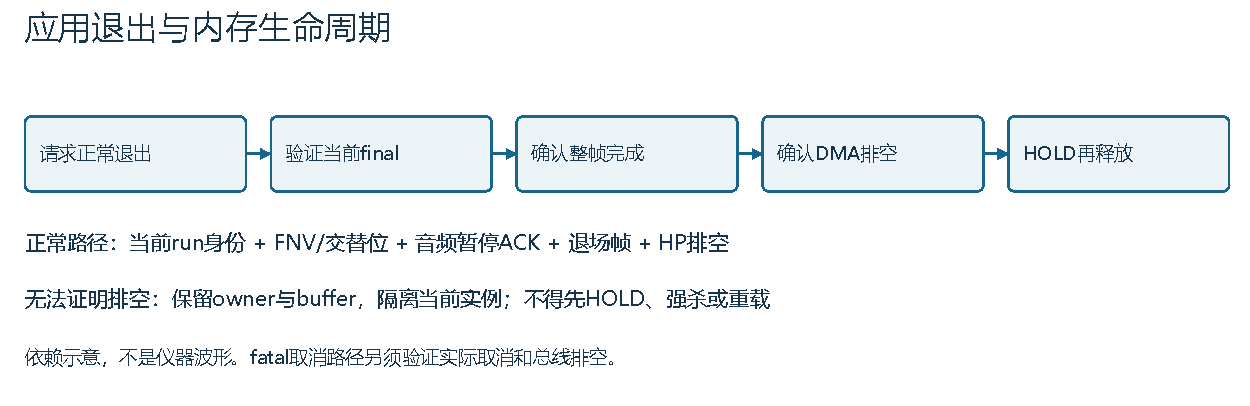
\includegraphics[width=\linewidth]{figures/owner_retirement.pdf}
\caption{应用退出与资源释放的依赖顺序}
\end{figure}

\Needspace{12\baselineskip}\section{优化过程与性能资源对比}

\Needspace{8\baselineskip}\subsection{测试方法与主要结果}

CoreMark 使用 GCC 13.3、RV32I\_Zmmul、O3 与 LTO，单核 2K 数据配置，4000 次迭代。性能轮记录 1129481426 个时钟周期，在 105 MHz 下对应 10.75696596 秒，得分 371.852；验证轮独立核对 CRC。图形帧率统计区分显示扫描与真正完成的新帧，持续 60 FPS 条件要求不少于 60 秒窗口内逐扫描提供新画面。\par

{\small\setlength{\tabcolsep}{4pt}\renewcommand{\arraystretch}{1.3}

\begin{longtable}{>{\raggedright\arraybackslash}p{0.2\linewidth}>{\raggedright\arraybackslash}p{0.38\linewidth}>{\raggedright\arraybackslash}p{0.34\linewidth}}

\toprule

\textbf{测试项目} & \textbf{实测结果} & \textbf{测试条件} \\ \midrule

\endfirsthead

\toprule

\textbf{测试项目} & \textbf{实测结果} & \textbf{测试条件} \\ \midrule

\endhead

CoreMark & 371.852 分；3.541 分/MHz & 105 MHz，4000 次；两配置 CRC 通过 \\

CoreMark/LUT & 0.05822 分/LUT（CPU核心） & 371.852064 分 / 6387 LUT \\

TILE & 3627 新帧 / 3627 扫描 & 512 对象，60.4500 秒 \\

DDR 位图 & 3625 新帧 / 3625 扫描 & 96 对象，60.4167 秒 \\

Alpha & 3625 新帧 / 3625 扫描 & 32 对象，60.4167 秒 \\

星际三挡 & 60.00 / 51.98 / 31.84 FPS & 密度 1 / 2 / 9；每挡不少于 60 秒 \\

鸡蛋三波 & 60.00 / 41.83 / 29.75 FPS & 64 / 85 / 100 对象；多个约 8 秒窗口 \\

\bottomrule

\end{longtable}

}

鸡蛋展示模式循环所选波次的 10 秒场景，排除前 2 秒预热后统计有效窗口；星际各挡采用不少于 60 秒的连续统计。三挡场景分别展示不同对象密度下的计算与绘制吞吐，形成可操作、可观察、可对照的负载梯度。\par

\begin{figure}[H]
\centering
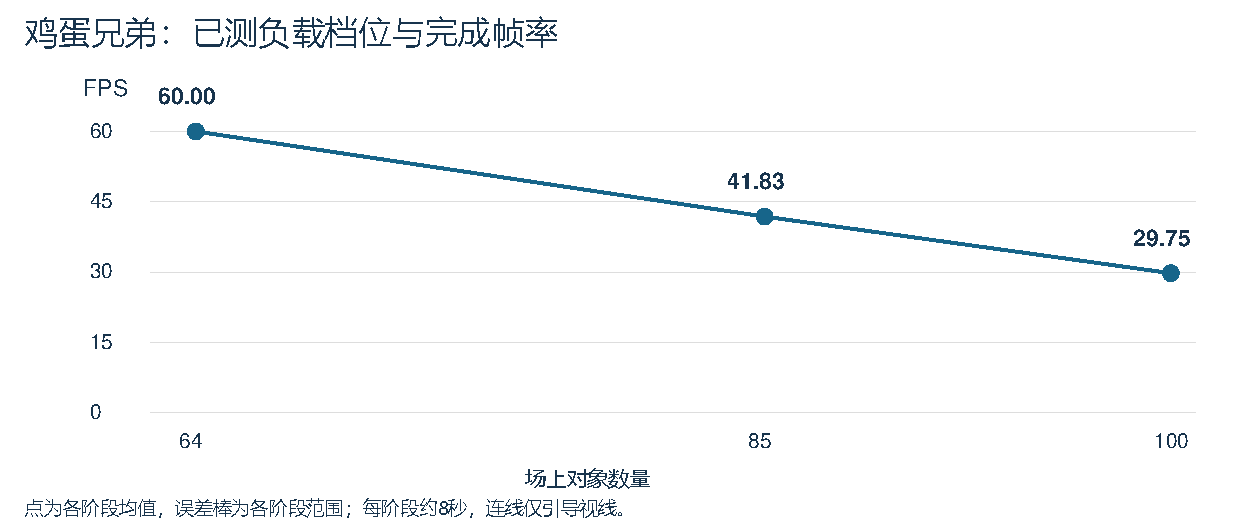
\includegraphics[width=\linewidth]{figures/egg_workload.pdf}
\caption{鸡蛋兄弟三档负载的有效计量窗口平均帧率}
\end{figure}

\Needspace{8\baselineskip}\subsection{优化方案与实现效果}

{\small\setlength{\tabcolsep}{4pt}\renewcommand{\arraystretch}{1.3}

\begin{longtable}{>{\raggedright\arraybackslash}p{0.2\linewidth}>{\raggedright\arraybackslash}p{0.38\linewidth}>{\raggedright\arraybackslash}p{0.34\linewidth}}

\toprule

\textbf{优化内容} & \textbf{优化前} & \textbf{采用方案及结果} \\ \midrule

\endfirsthead

\toprule

\textbf{优化内容} & \textbf{优化前} & \textbf{采用方案及结果} \\ \midrule

\endhead

帧存组织 & 完整画布需 480000 字节 & 两带顺序复用 262144 字节暂存区，完成原生 800×600 绘制与整帧提交 \\

程序加载 & 菜单出现前集中准备资源，软件重启约 40～43 秒 & 按需加载并缓存，软件重启两次分别 33.38 / 36.10 秒；首次应用进入约 2.7～4.6 秒，重复约 0.4～0.6 秒 \\

音频补给 & Python 逐样本写 FIFO 增加解释器开销 & 同一管理进程调用 C 函数连续写入，PCM 校验确认对应输出数据一致 \\

应用切换 & 多模块分别管理退出与资源 & 统一退出握手与搬运完成链，通过仿真和实机切换验证有序交接 \\

\bottomrule

\end{longtable}

}

按需加载与缓存复用将软件重启至菜单的时间由约 40～43 秒缩短至 33.38～36.10 秒，重复进入应用约需 0.4～0.6 秒。处理器执行、存储访问、图形绘制与运行管理的优化分别通过对应的周期、帧率、资源及启动数据评价，构成从微架构到交互体验的协同优化。\par

\Needspace{8\baselineskip}\subsection{资源与时序}

{\small\setlength{\tabcolsep}{4pt}\renewcommand{\arraystretch}{1.3}

\begin{longtable}{>{\raggedright\arraybackslash}p{0.23\linewidth}>{\raggedright\arraybackslash}p{0.14\linewidth}>{\raggedright\arraybackslash}p{0.14\linewidth}>{\raggedright\arraybackslash}p{0.2\linewidth}>{\raggedright\arraybackslash}p{0.17\linewidth}}

\toprule

\textbf{范围} & \textbf{LUT} & \textbf{FF} & \textbf{BRAM36} & \textbf{DSP} \\ \midrule

\endfirsthead

\toprule

\textbf{范围} & \textbf{LUT} & \textbf{FF} & \textbf{BRAM36} & \textbf{DSP} \\ \midrule

\endhead

完整 PL 系统 & 23447 & 11576 & 126 & 4 \\

CPU 核心 & 6387 & 2081 & 0 & 4 \\

\bottomrule

\end{longtable}

}

CPU 核心包含 5998 个逻辑 LUT 与 389 个 LUTRAM，共 6387 LUT；外部缓存、工作 RAM、图形和显示模块按各自层级统计。CPU 资源效率为 371.852064 ÷ 6387 = 0.05822 CoreMark/LUT。完整 PL 为 23447 LUT，占器件 LUT 的约 44.07\%。105 MHz 实现后 WNS +0.033 ns、WHS +0.057 ns、WPWS +0.312 ns，满足实现时序要求。\par

\Needspace{12\baselineskip}\section{大模型协作记录与设计复盘}

模型参与需求分析、源码检查、RTL/C/Python 实现、实验脚本及结果整理。参赛者负责设计目标、接线、实物操作、效果判断和方案取舍。协作按“分析实际输入—提出方案—实现—独立参考比对—板端验证”组织，生成结果必须经过验证后才能进入稳定工程。\par

协作材料按“原始交互节选—设计归纳—验证记录”组织。collaboration 目录保存带来源定位的提示词与回答，model\_collaboration.md 汇总方法与结论。典型优化过程如下。\par

{\small\setlength{\tabcolsep}{4pt}\renewcommand{\arraystretch}{1.3}

\begin{longtable}{>{\raggedright\arraybackslash}p{0.2\linewidth}>{\raggedright\arraybackslash}p{0.38\linewidth}>{\raggedright\arraybackslash}p{0.34\linewidth}}

\toprule

\textbf{优化任务} & \textbf{设计判断与实现} & \textbf{验证方法} \\ \midrule

\endfirsthead

\toprule

\textbf{优化任务} & \textbf{设计判断与实现} & \textbf{验证方法} \\ \midrule

\endhead

多模块资源交接 & 根据生产者与消费者依赖统一退出顺序 & RTL 正负例、退出状态核验与板端切换 \\

不同绘制吞吐下的遥测接收 & 联合管理持续进展与整包时间窗口 & 慢速封包回放、负例及真实板端记录 \\

综合资源与测试结果关联 & 按顶层实例、二进制与原始报告绑定 & 文件哈希、原始计数与独立重算 \\

\bottomrule

\end{longtable}

}

协作实践提高了跨模块关系梳理、方案比较和重复验证脚本的编写效率。模型建议经过源码核对、仿真和板端测试形成工程实现，实物操作进一步验证输入、显示与音频的协同效果。\par

\Needspace{12\baselineskip}\section{技能包提炼过程与验证}

项目围绕可复现构建、独立结果核对和应用资源交接，提炼了产物身份与二进制范围校验、PYNQ 资源生命周期管理两类可复用方法。skill 目录提供 README、使用步骤和适用条件，便于其他工程直接采用。\par

产物校验工具仅依赖 Python 标准库，接收清单、文件路径及比较范围，先核对非空输入与边界，再比较实际字节。验证覆盖正常、坏哈希、坏字节、空范围、越界、路径逃逸、空清单和合法局部比较八类情况，并对工程公开快照执行身份核对。\par

生命周期方法按“停止请求—生产者完成—消费者排空—释放资源”分析依赖，将可复用控制顺序与作品专用地址和寄存器配置分离。迁移时依据目标硬件的缓存、DMA 与外设协议补充配置及对应测试，既保留通用方法，也便于适配不同工程。\par

\Needspace{12\baselineskip}\section{复现说明}

\Needspace{8\baselineskip}\subsection{环境与工程组织}

硬件工具为 Vivado 2025.2.1，目标 XC7Z020CLG400-2；RV32 编译器为 GCC 13.3。板端需具备匹配 AX7020 的 PYNQ/Linux 环境及对应显示、USB 与音频连接。工程中的 software、hardware、runtime、sim、verification、skill、report 分别保存应用源码、硬件输入、运行入口、仿真、原始测量、技能包和报告。\par

\Needspace{8\baselineskip}\subsection{构建与校验步骤}

1. 从提交工程根目录读取 README、运行环境与来源清单，使用新的输出目录，核对 manifest 所登记的输入文件。\par

2. 执行 python software/rebuild.py --destination <new\_dir> --compiler <gcc\_path>，生成八个 RV32 程序并核对预期二进制。\par

3. 执行 python hardware/rebuild.py --destination <new\_dir> --vivado <vivado\_path>，从 RTL、XDC、IP/BD 和初始化数据重建硬件，检查资源与时序报告。\par

4. 执行 python sim/replay.py --destination <new\_dir> --vivado-bin <vivado\_bin>，重放功能正负例；再运行 verification 中的重算脚本核对性能与像素记录。\par

5. 按 runtime/readme.md 配置板端环境，确认没有其他进程占用硬件后启动 runtime/run.py --start，检查菜单、应用、输入、音频与正常退出。\par

以上步骤的完整命令、依赖版本和输出位置见 reproduction.md。工程已完成八程序独立重建及二进制一致性核对，并提供硬件源码综合、布局布线、导出记录与对应板端实测数据。源代码、构建配方、运行载荷和验证结果通过文件清单关联，为作品复现与继续开发提供完整入口。\par

\clearpage\section{参考文献}

[1] AMD. 全国大学生嵌入式芯片与系统设计竞赛 FPGA 赛道选题指南，2026，第 3.3 节.\par

[2] EEMBC. CoreMark. https://github.com/eembc/coremark.\par

[3] YosysHQ. PicoRV32. https://github.com/YosysHQ/picorv32.\par

[4] Project F. FPGA Graphics and Display Designs. https://github.com/projf/projf-explore.\par

[5] Xilinx. PYNQ. https://github.com/Xilinx/PYNQ.\par

[6] Digilent. Vivado Library RGB to DVI IP. https://github.com/Digilent/vivado-library.\par

[7] strigeus. fpganes. https://github.com/strigeus/fpganes.\par

[8] Kenney. Space Shooter Remastered. https://kenney.nl/assets/space-shooter-remastered.\par

\end{document}
